\documentclass[10pt]{article}
\usepackage[margin=0.55in]{geometry}
\usepackage{amsmath,amssymb}
\usepackage{tikz}
\usetikzlibrary{arrows.meta,positioning}
\usepackage{enumitem}
\usepackage{titlesec}
\usepackage{microtype}
\pagestyle{empty}
\setlength{\parindent}{0pt}
\setlength{\parskip}{3pt}
\titlespacing*{\section}{0pt}{5pt}{2pt}
\titleformat{\section}{\bfseries\normalsize}{\thesection}{0.4em}{}
\setlist[itemize]{leftmargin=1.1em,itemsep=0pt,topsep=1pt}

\begin{document}

\begin{center}
{\Large \textbf{Reward-Conditioned Reverse Diffusion for Portfolio Optimization}}\\
Siddhant Sukhani \quad MS\&E 342 \quad Instructor: Prof. Renyuan Xu \quad Final report due: June 12, 2026
\end{center}

\section*{Objective}
This project studies whether a score-based diffusion model for financial return scenarios can be fine-tuned through KL-penalized stochastic control so that generated scenarios remain distributionally realistic while becoming more useful for downstream portfolio decisions. Existing diffusion-based finance papers typically train a generative model to match historical returns and then pass generated scenarios to a portfolio optimizer. The portfolio objective does not feed back into the generator. This project addresses that decoupling by adding a controlled perturbation to the reverse SDE drift and optimizing a terminal portfolio reward subject to a KL penalty relative to the base model.

\section*{Method}
The base model is a variance-preserving SDE trained by denoising score matching on daily log returns for 10 S\&P 500 sector ETFs. Generation follows the reverse SDE
\[
dY_t=\left[-\frac{\beta(T-t)}{2}Y_t+\beta(T-t)s_\theta(Y_t,T-t)\right]dt+\sqrt{\beta(T-t)}d\widetilde W_t.
\]
Fine-tuning introduces a control $u_\phi(Y_t,t)$ and solves
\[
\max_{\phi}\ \mathbb{E}_{p_\phi}[U(Y_T)]-\eta\,\mathrm{KL}(p_\phi\|p_\theta).
\]
By Girsanov's theorem, the KL term becomes a quadratic control cost. The associated HJB equation is
\[
\partial_t V+\mathcal{L}^{s_\theta}V+\frac{\beta(T-t)}{2\eta}\|\nabla_y V\|^2=0,\qquad V(T,y)=U(y).
\]

\section*{Pipeline}
\begin{center}
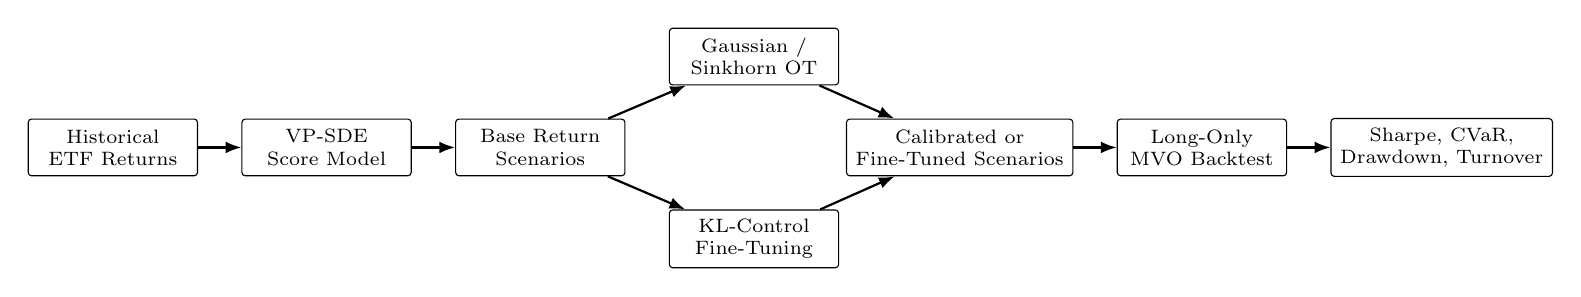
\begin{tikzpicture}[
  node distance=0.55cm and 0.55cm,
  box/.style={draw, rounded corners=1.2pt, align=center, minimum width=2.15cm, minimum height=0.72cm, font=\scriptsize},
  arrow/.style={-{Latex[length=2mm]}, thick}
]
\node[box] (data) {Historical\\ETF Returns};
\node[box, right=of data] (score) {VP-SDE\\Score Model};
\node[box, right=of score] (base) {Base Return\\Scenarios};
\node[box, above right=0.42cm and 0.55cm of base] (ot) {Gaussian /\\Sinkhorn OT};
\node[box, below right=0.42cm and 0.55cm of base] (ctrl) {KL-Control\\Fine-Tuning};
\node[box, right=2.8cm of base] (scen) {Calibrated or\\Fine-Tuned Scenarios};
\node[box, right=of scen] (mvo) {Long-Only\\MVO Backtest};
\node[box, right=of mvo] (metrics) {Sharpe, CVaR,\\Drawdown, Turnover};
\draw[arrow] (data) -- (score);
\draw[arrow] (score) -- (base);
\draw[arrow] (base) -- (ot);
\draw[arrow] (base) -- (ctrl);
\draw[arrow] (ot) -- (scen);
\draw[arrow] (ctrl) -- (scen);
\draw[arrow] (scen) -- (mvo);
\draw[arrow] (mvo) -- (metrics);
\end{tikzpicture}
\end{center}

\section*{Empirical Design}
The data will be split into 2014-2020 for score-model training, 2021 for validation and $\eta$ selection, and 2022-2024 for final testing. Strategies include equal weight, rolling Markowitz, Wasserstein-robust MVO, base diffusion scenarios, Gaussian OT calibrated scenarios, and KL-fine-tuned diffusion scenarios. Metrics include Sharpe ratio, CVaR(95\%), maximum drawdown, turnover, and portfolio concentration.

\section*{Contributions and Expected Findings}
\begin{itemize}
\item \textbf{Theory:} derive the HJB optimality condition and a closed-form linear-Gaussian benchmark where $u^*(t,y)=\beta(T-t)\nabla V(t,y)/\eta$.
\item \textbf{Calibration:} quantify how Gaussian OT and Sinkhorn-based calibration affect generated means, covariances, and portfolio weights.
\item \textbf{Empirics:} estimate an $\eta$ frontier that measures the trade-off between distributional realism and decision usefulness.
\end{itemize}
Preliminary results show that the base diffusion model underestimates volatility and produces overly concentrated portfolios, while Gaussian OT restores first and second moments and recovers diversified weights. The final project will present these results as an interpretable realism-performance frontier, not as a statistically decisive outperformance claim.

\end{document}
